\section{Bezprzewodowy system monitoringu parametrów jakości powietrza}
\label{system}

\subsection{Technologia IQRF}

IQRF jest to bezprzewodowa technologia Mesh pracująca w pod-gigaherzowych pasmach ISM. Nie wymaga żadnej zewnętrznej infrastruktury, 
licencji i opłat dostawcy \cite{what-iqrf}. Zamontowanie transceivera IQRF w kompatybilnych urządzeniach pozwala im na komunikację między sobą
poprzez przesyłanie pakietów danych. 

Każda sieć wykorzystująca IQRFMESH potrzebuje koordynatora do odpowiedniego działania. Urządzenia w sieci komunikują się na zasadzie
master(koordynator) - slave(węzeł). Węzły nie mogą komunikować się ze sobą bezpośrednio, natomiast w topologi innej niż
Gwiazda (np. Mesh) węzły wspierają routowanie pakietów do innych węzłów \cite{iqrf-rules}.

IQRFMESH jest protokołem umożliwiającym, między innymi, zwiększenie zasięgu sieci poprzez umożliwienie węzłom routowania pakietów.
Jest możliwe połączenie urządzeń bez wykorzystania tego protokołu, ale na potrzeby tej pracy jest to zalecane \cite{iqrfmesh}. Urządzenia w 
sieci IQRFMESH komunikują się poprzez protokół DPA, w której wiadomości są przesyłane w strukturze bajtowej \cite{dpa-guide}.

Każda z wiadomości przesyłanych protokołem składa się co najmniej z:
\begin{itemize}
    \item NADR - 2-bajtowy adres urządzenia docelowego
    \item PNUM - 1-bajtowy adres urządzenia peryferialnego w urządzeniu docelowym. Peryferium może być na przykład czujnik temperatury bądź wbudowana dioda LED
    \item PCMD - 1-bajtowa komenda, której wykonanie zleca się urządzeniu. 
    \item HWPID - 1-bajtowy Identyfikator Profilu Urządzenia (HardWare Profile ID). Wartość stała określająca rodzaj/model urządzenia. Dla wykorzystywanych w projekcie
czujników jest to "4001".
\end{itemize}

oraz opcjonalnie z pola DATA, które może zawierać maksymalnie 56 bajtów danych. Cała wiadomość, łącznie z obowiązkowymi parametrami wymienionymi wyżej nie może przekroczyć
64 bajtów 

Przykład wiadomości:

\begin{center}
    \textbf{01005E010140FFFFFFFF}
\end{center}

jeżeli rozdzielimy ją na poszczególne parametry uzyskujemy:

\begin{table}[h]
    \centering
    \begin{tabular}{|c|c|c|c|c|}
    \hline
    NADR & PNUM & PCMD & HWPID & DATA \\ \hline
    0100 & 5E & 01 & 0140 & FFFFFFFF \\ \hline
    \end{tabular}
\end{table}

Protokół DPA stosuje ustawienie bajtów typu little-endian. W związku z tym bajty każdego parametru dłuższego
niż 2 bajty są pisane "od końca". Przykładowo, jeżeli chcemy zaadresować urządzenie o NADR równym "0001", to 
do ramki wiadomości odpowiadającej temu adresowi wpisuje się "0100". Taka sama sytuacja ma miejsce z parametrem
HWPID, który również ma długość większą niż 1 bajt.

Powyższa wiadomość pochodzi z dokumentacji czujnika Protronix używanego w projekcie \cite{protronix-comms}, a jej 
wysłanie powoduje zebranie z czujnika o adresie 0001 danych ze wszystkich dostępnych czujników - temperatury, 
wilgotności, dwutlenku węgla i baterii, jeżeli jej stan jest niski.

\subsection{Czujniki i bramka IQRF}

Urządzeniami bezpośrednio odpowiedzialnymi za pobieranie z otoczenia danych o jakości powietrza są cztery czujniki NLB-CO2+RH+T-5-IQRF firmy
Protronix (Rys. \ref{czujnik}). Każdy czujnik jest w stanie odczytać temperaturę, wilgotność względną oraz zawartość dwutlenku węgla w powietrzu. Zasilanie jest zapewniane
bateryjnie poprzez dwie baterie AA 1.5V, a komunikacja odbywa się poprzez zamontowany w gnieździe SIM nadajnikoodbiornik (transceiver) IQRF.
Każdy taki sensor stanowi węzeł sieci IQRFMESH.

\begin{figure}[H]
    \centering
    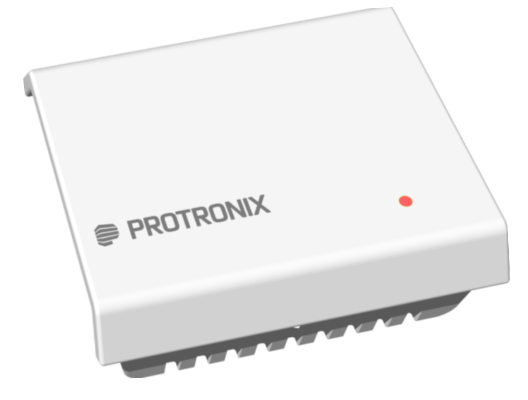
\includegraphics[width=0.5\textwidth]{zdj/NLB-CO2RHT-5-IQRF.jpg}
    \caption{Podglądowe zdjęcie wykorzystywanego czujnika \cite{protronix-product}}
    \label{czujnik}
\end{figure}

Koordynatorem sieci jest bramka GW-ETH02 (Rys. \ref{bramka}) zasilana sieciowo napięciem 5VDC. Urządzenie łączy się z Internetem poprzez gniazdo Ethernet oraz
posiada gniazdo karty SD jako jedną z opcji zapisu danych. Bramka posiada wbudowany transceiver IQRF.

\begin{figure}[H]
    \centering
    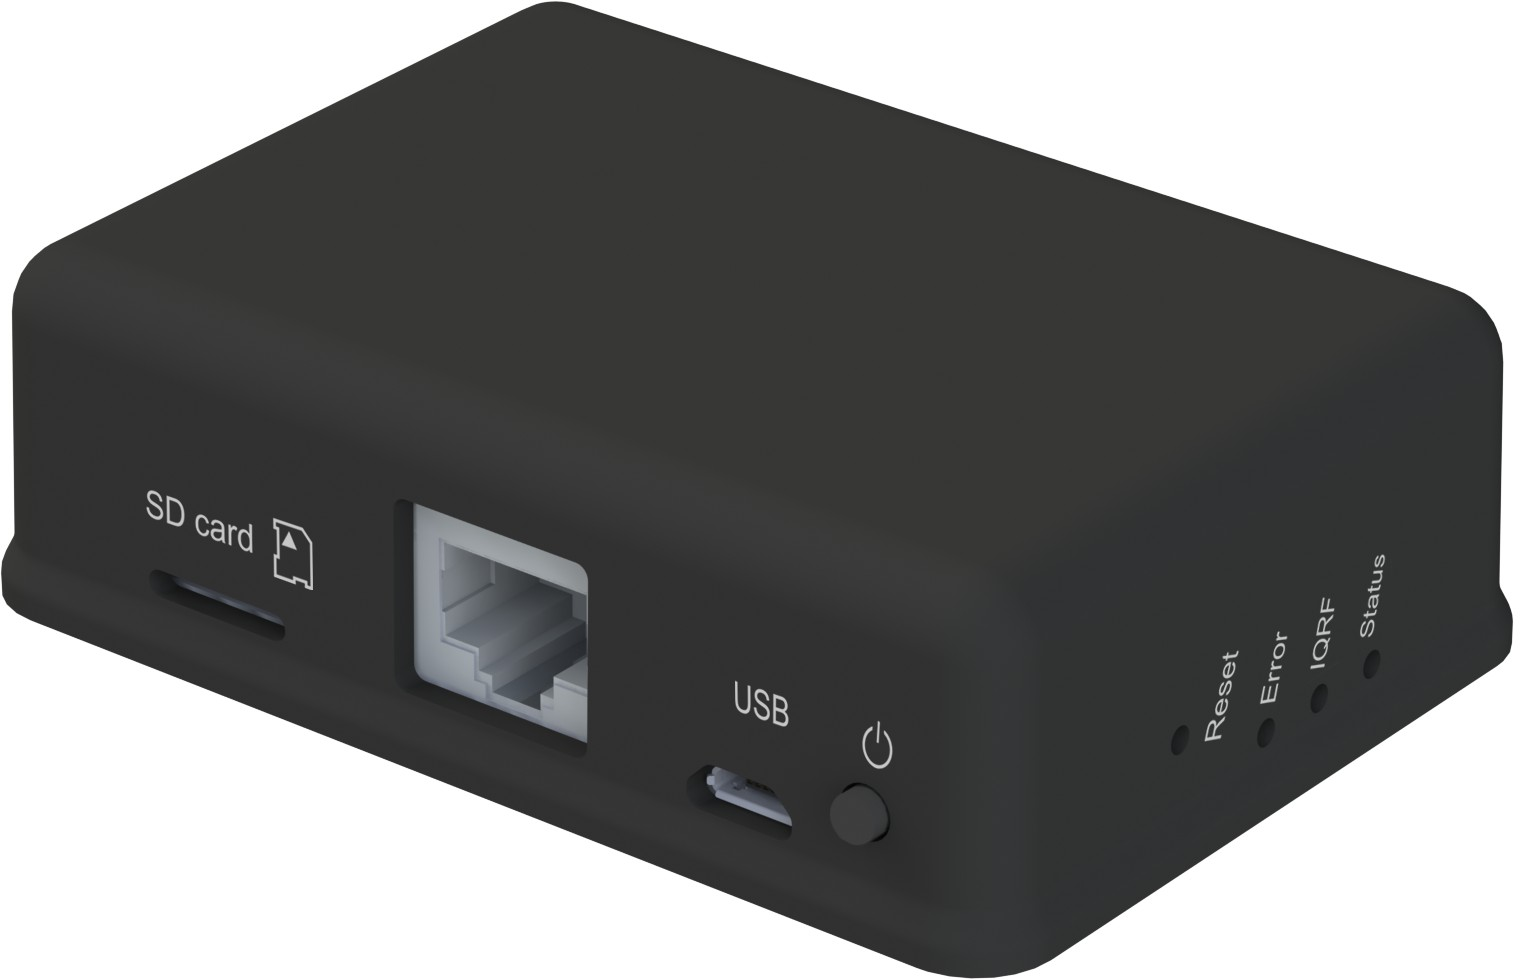
\includegraphics[width=0.5\textwidth]{zdj/gateway.png}
    \caption{Podglądowe zdjęcie bramki \cite{gateway-product}}
    \label{bramka}
\end{figure}

\subsubsection{Konfiguracja}

Do konfiguracji urządzeń wchodzących w skład sieci posłużono się narzędziem IQRF IDE w wersji 4.70. Narzędzie to umożliwia między 
innymi konfigurację modułów IQRF TR zawartych w urządzeniach oraz odczyt pewnych danych o transceiverach IQRF, takich jak wersja systemu
operacyjnego czy protokołu DPA.

Bramka może pracować w dwóch trybach: Datalogger lub Gateway. Konfiguracja bramki jako Datalogger powoduje przesłanie wszystkich danych,
wchodzących i wychodzących, do serwera IQRF Cloud. Z kolei konfiguracja bramki jako Gateway nie pozwala na korzystanie z IQRF Cloud, za to wymaga 
zdalnego połączenia przez protokół UDP z urządzeniem końcowym.

Jako, iż serwer IQRF Cloud zapewnia wygodę w postaci dobrze udokumentowanego API, możliwości interakcji z bramką z poziomu strony oraz swego
rodzaju buffer w postaci 2000 rekordów, w pracy zdecydowano się użyć ustawienia Datalogger.

Tego jak i innych potrzebnych ustawień można dokonać wybierając opcje TR Configuration w IQRF IDE podczas, gdy bramka jest fizycznie podłączona
do komputera. Parametry bramki zostały ustawione na wartości przewidziane przez producenta czujników Protronix \cite{protronix-comms}. Upewniono 
się również, że bramka będzie działała z urządzeniami LP (Low Power), poprzez wybranie na panelu odpowiedniego ustawienia sieci STD+LP.

Następnie każdy z transceiverów przeznaczonych do montażu w czujnikach został tymczasowo zamontowany w programatorze CK-USB-04A będącego częścią
zestawu IoT Starter Kit w celu sprawdzenia poprawności ustawień transceivera zgodnie z zaleceniami producenta (Rys. \ref{fab-conf}).

\begin{figure}[H]
    \centering
    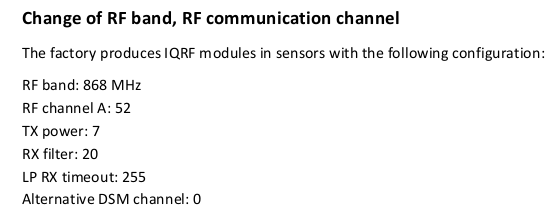
\includegraphics[width=0.7\textwidth]{zdj/protronix-settings.png}
    \caption{Fabryczna konfiguracja modułów TR. Wycinek z \cite{protronix-comms}}
    \label{fab-conf}
\end{figure}

\subsubsection{Topologia sieci}

To, w jakiej topologii będą pracowały czujniki sieci IQRF MESH zależy od odległości między czujnikiem a bramką. W przypadku 
mniejszych dystansów wszystkie czujniki będą bezpośrednio połączone bezprzewodowo z bramką - topologia gwiazdy. Jeżeli natomiast
odległości są znaczne niektóre węzły sieci mogą sprawować również funkcję routerów, przekierowujących pakiety między innymi 
węzłami i bramką. W takim przypadku mamy do czynienie z topologią siatki (Rys. \ref{topologies}).

\begin{figure}[H]

\centering
\begin{subfigure}{0.4\textwidth}
    \centering
    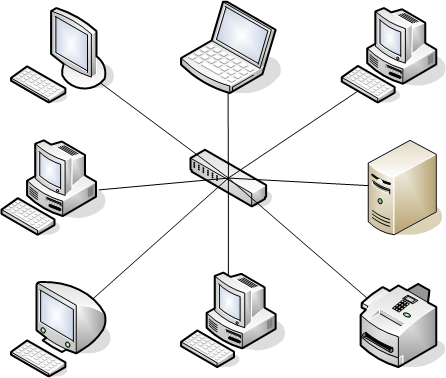
\includegraphics[width=0.8\linewidth]{zdj/star-top.png}
    \caption{Topologia gwiazdy \cite{fig-star-top}}
\end{subfigure}
\begin{subfigure}{0.4\textwidth}
    \centering
    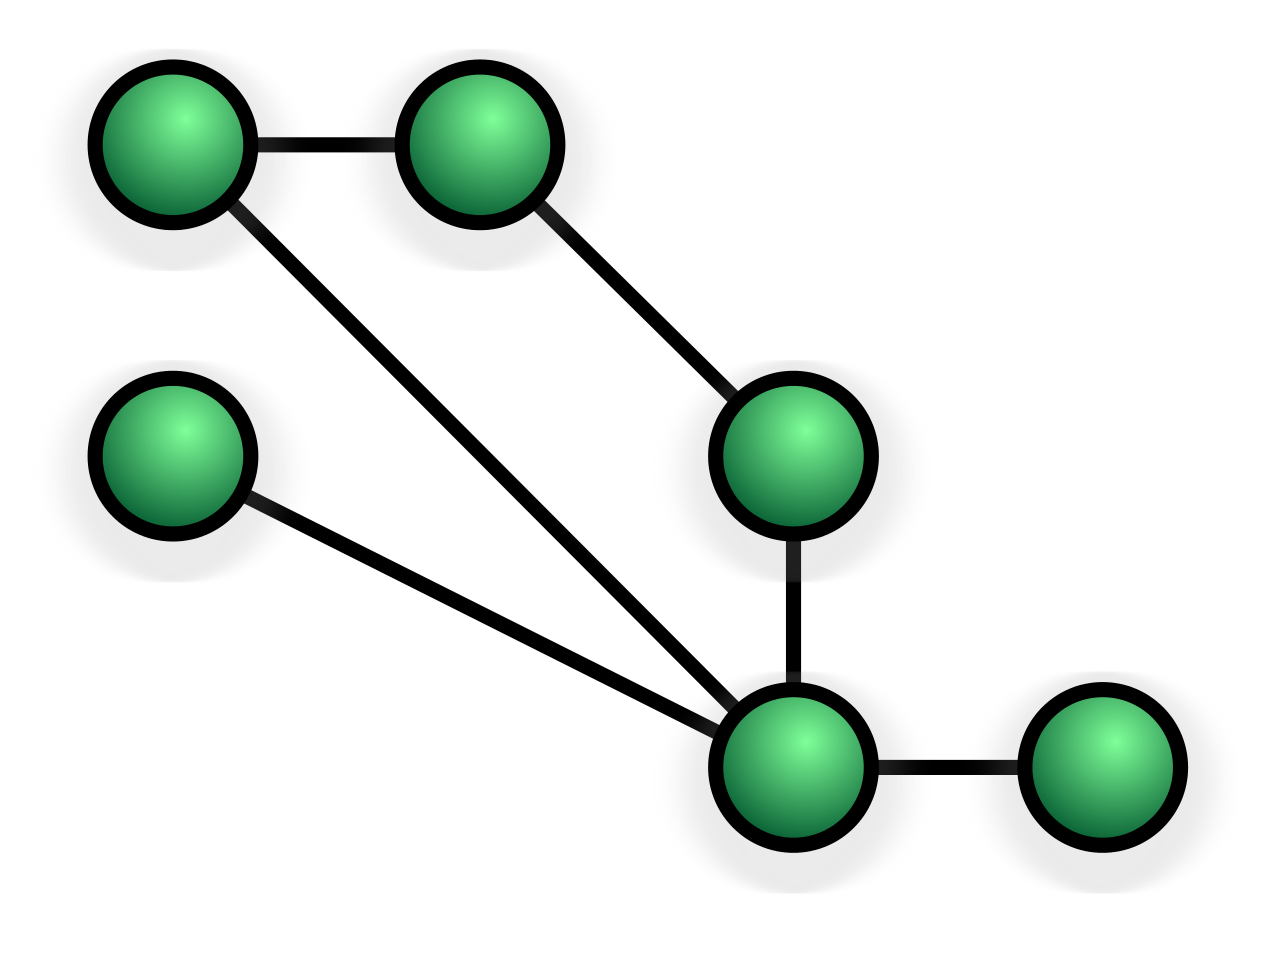
\includegraphics[width=0.8\linewidth]{zdj/mesh-top.png}
    \caption{Topologia siatki \cite{fig-mesh-top}}
\end{subfigure}
   
\caption{Schematy porównujące obie topologie sieci}
\label{topologies}

\end{figure}

Dzięki dosyć małej odległości od siebie i od bramki udało się uzyskać topologię gwiazdy.

\subsection{Serwer IQRF Cloud}

IQRF Cloud jest serwisem w chmurze umożliwiającym komunikację z bramką IQRF po jej zarejestrowaniu w tymże serwisie, w którym uprzednio należy
założyć konto. Po rejestracji serwis umożliwia obustronną komunikację z urządzeniem w postaci wiadomości protokołu DPA. Aby takową nadać należy 
wejść w panel zarejestrowanej bramki i wybrać opcję 'Send command to gateway' (Rys. \ref{send-comm}):

\begin{figure}[H]
    \centering
    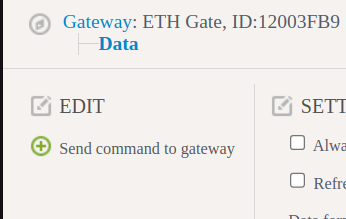
\includegraphics[width=0.4\textwidth]{zdj/send-command-to-gw.png}
    \caption{Opcja "Send command to gateway"}
    \label{send-comm}
\end{figure}

Po wybraniu tej opcji otrzymujemy widok umożliwiający wysyłanie do brami wiadomości protokołem DPA, a każde nadanie wymaga dodatkowo podania
hasła do bramki wybieranego na etapie konfiguracji (Rys. \ref{send-data}).

\begin{figure}[H]
    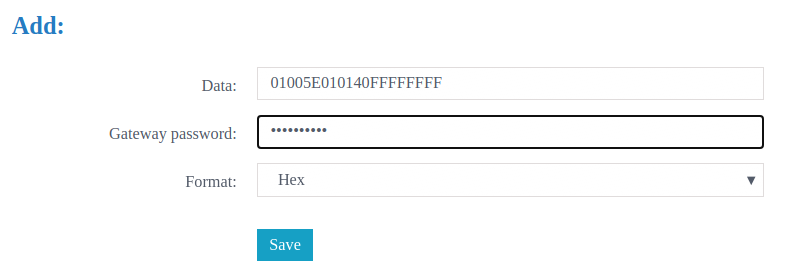
\includegraphics[width=\textwidth]{zdj/cloud-send-message.png}
    \caption{Fragment panelu umożliwiający wysłanie danych z serwera chmury do bramki}
    \label{send-data}
\end{figure}

Dane odbierane/wysyłane przez serwer i bramkę są widoczne w panelu głównym odpowiednim dla bramki. Na serwerze może istnieć jednocześnie tylko 2000
rekordów. Po przekroczeniu tego limitu najstarsze dane są nadpisywane.

Każdy rekord skład się z:
\begin{itemize}
    \item indeksu 
    \item czasu otrzymania przez serwer i bramkę
    \item kierunku przesyłu danych (transmisja a odbiór)
    \item długości danych wyrażonej w bajtach 
    \item samych danych w formacie szesnastkowym (znaki 0-9 i A-F)
    \item statusu odebrania przez bramkę (Sent, Confirmed, Expired...)
    \item indeksu w bazie danych serwera.
\end{itemize}

\begin{figure}[H]
    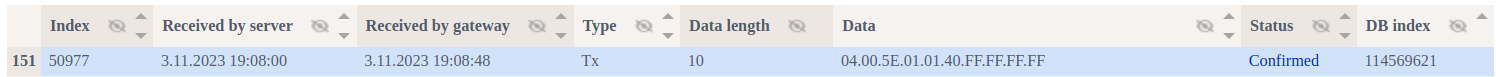
\includegraphics[width=\textwidth]{zdj/cloud-records.png}
    \caption{Fragment tabeli otrzymanych wiadomości w IQRF Cloud}
    \label{records-frag}
\end{figure}

Widok pokazany na Rys. \ref{records-frag} stanowi jednak dla tej pracy bardziej narzędzie diagnostyczne niż kluczowy element działania systemu - z poziomu działania aplikacji
webowej nie da się wejść w interakcję z tym panelem, a przynajmniej nie jest to przewidziane. Serwis udostępnia więc własny interfejs 
programistyczny (API), który umożliwia przesyłanie zapytań z innego urządzenia do tego serwisu i w konsekwencji do bramki oraz czujników.

Każde zapytanie wysyłane do serwera składa się z adresu bazowego na jaki przesyłamy zapytania, wymaganych i opcjonalnych parametrów oraz tzw. 
sygnatury. Adresem bazowym na dzień pisania pracy jest \textbf{https://cloud.iqrf.org/api/api.php?}.

\subsubsection{Parametry wymagane i opcjonalne}

Lista parametrów wymaganych prezentuje się następująco:

\begin{itemize}
    \item ver - aktualna wersja API. W trakcie pisania pracy jest to "2" 
    \item uid - login użytkownika do serwisu IQRF Cloud
    \item gid - ID zarejestrowanej bramki, z którą chcemy się komunikować. Widoczne zarówno w portalu jak i na obudowie bramki
    \item gpw - hasło do bramki. Wymagane jedynie w przypadku stosowania komendy "add"
    \item cmd - jedna z komend: dnld, uplc, dnlc
    \item data - dane do przesłania do bramki
    \item signature - podpis potwierdzający użytkownika.
\end{itemize}

Parametry opcjonalne dają zaś kontrolę nad ilością pobieranych danych:

\begin{itemize}
    \item from - indeks pierwszego rekordu, który chcemy pobrać
    \item to - indeks ostatniego rekordu, który chcemy pobrać
    \item count - ilość pobieranych rekordów
    \item time\_from - data utworzenia pierwszego rekordu, który chcemy pobrać 
    \item time\_to - data utworzenia ostatniego rekordu, który chcemy pobrać
    \item new - pobieranie danych zaczynając od ostatniego pobranego rekordu
    \item last - pobieranie rekordów zaczynając od najpóźniejszych
\end{itemize}

Bardziej szczegółowy opis wszystkich parametrów oraz ograniczenia w ich stosowaniu dostępne są w dokumentacji IQRF Cloud Serwer Technical Guide 
\cite{iqrfcloud-guide}

\subsubsection{Sygnatura zapytania}

Jakakolwiek komunikacja z serwerem wymaga podania parametru \textbf{signature}, który gwarantuje bezpieczeństwo przesyłu danych przez API 
potwierdzając prawo dostępu użytkownika do danych. Dokumentacja \cite{iqrfcloud-guide} definiuje sygnaturę następująco:

\begin{figure}[H]
    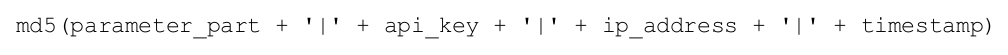
\includegraphics[width=\textwidth]{zdj/md5.png}
\end{figure}

Gdzie: 


\begin{itemize}
    \item parameter\_part - ciąg znaków adresu URL zapytania pomiędzy adresem bazowym a sygnaturą. Na przykład, dla zapytania \\
    'https://cloud.iqrf.org/api/api.php?ver=2\&uid=xx\&gid=xx\&cmd=dnld\&signature=xx \\
wartość ta jest równa "ver=2\&uid=xx\&gid=xx\&cmd=dnld'
    \item api\_key - klucz API dostępny po zalogowaniu się do portalu IQRF Cloud (Rys. \ref{api-key})
    \item ip\_address - adres IP klienta
    \item timestamp - liczba sekund począwszy od 01.01.1970 00:00UTC podzielona przez 600. Podzielenie przez 600 zapewnia 10-minutową
ważność każdej sygnatury.
\end{itemize}

'md5' jest zaś kryptograficzną funkcją haszującą, której argumentem jest wyżej przedstawiony ciąg znaków 


\begin{figure}[H]
    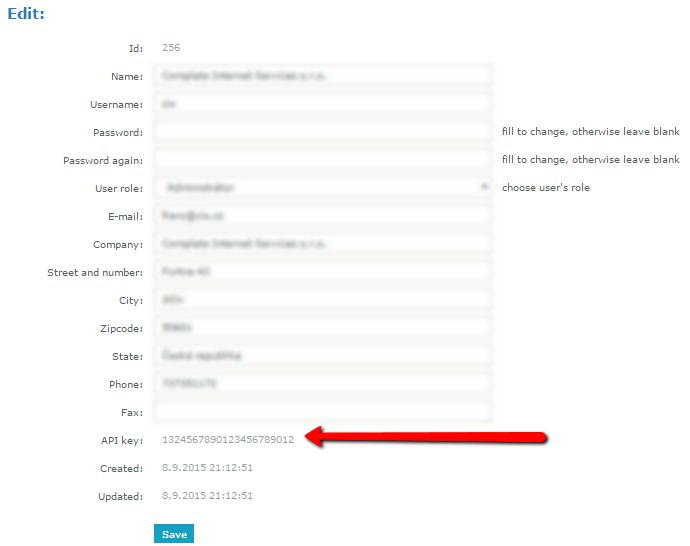
\includegraphics[width=\textwidth]{zdj/api-key.png}
    \caption{Fragment widoku profilu użytkownika. Czerwoną strzałką wskazano klucz API.}
    \label{api-key}
\end{figure}

Kompletne zapytanie składa się z adresu bazowego, ciągu parametrów oraz sygnatury. Na przykład:
\begin{center}
    \begin{small}
        https://cloud.iqrf.org/api/api.php?ver=2\&uid=12345678\&gid=ABCD1234\&cmd=dnld\&signature=x
    \end{small}
\end{center}

jest ważnym zapytaniem API i spowoduje pobranie maksymalnie 500 rekordów z serwera, zakładając poprawność wszystkich parametrów.

\subsection{Aplikacja webowa}

Aplikacja webowa stanowi centralny obiekt tej pracy i jest ostatnim elementem wchodzącym w skład systemu monitorowania danych
z czujników. 

Serwer tej aplikacji jest odpowiedzialny za wysyłanie zapytań do serwisu IQRF Cloud w celu poboru danych z czujników, pobieranie
tych danych z serwisu, walidacje, filtrowanie, formatowanie i zapisywanie do bazy danych. Zapewnia również szereg ścieżek API pozwalających
klientowi na interakcje z zasobami zapisanymi w bazie danych (odczyty z czujników i ich metadane). Zastosowanie bazy danych 
jest konieczne ze względu na fakt, że serwis IQRF Cloud przechowuje tylko 2000 najnowszych rekordów.

Klient natomiast zapewnia czytelny interfejs graficzny w postaci szeregu widoków umożliwiających przeglądanie aktualnych i 
historycznych danych oraz ich pobieranie.

Dokładniejszy opis działania aplikacji webowej zostanie przedstawiony w dalszej części pracy.

\subsection{Opis działania całego systemu}

Typowy cykl działania systemu jest wywoływany co 5 minut, a prezentuje się on następująco:

\begin{enumerate}
    \item Serwer aplikacji wysyła zapytanie do IQRF Cloud o pobranie danych z czujników.
    \item IQRF cloud otrzymuje zapytanie o odczyt czujników i przekazuje je do bramki
    \item Czujniki otrzymują wiadomość przesłaną przez bramkę i odsyłają odczyt z czujników z powrotem do bramki
    \item Bramka przesyła odczyty do serwera IQRF Cloud gdzie są tymczasowo zapisywane.
    \item Serwer aplikacji webowej wysyła kolejne zapytanie, tym razem o przesłanie danych z IQRF cloud
do aplikacji.
    \item Dane pobrane na serwer aplikacji są kolejno poddawane walidacji, filtrowaniu i formatowaniu.
    \item Przygotowane dane są zapisywane w bazie danych 
    \item Klient pobiera nowe dane z bazy
    \item Dane prezentowane na widokach ulegają odświeżeniu pod wpływem zmiany dostępnych danych.
\end{enumerate}